\problemname{Snow Chaos}
A snowstorm has arrived and traffic is in chaos.
On top of that, certain sections of the railway track have been snowed in, causing all train traffic to stop.
This is naturally not very good, since lots of travelers are now standing at their stations unable to get anywhere.
Fredrika has therefore been tasked with clearing the snow between the stations before rush hour begins and disaster strikes.

The railway track has no branches and has $n$ stations, numbered from $1$ to $n$ in the order they appear on the track (so that station $i$ comes right before station $i+1$).
There are thus $n - 1$ sections between the stations.
Of these, $s$ are covered with snow.

Fredrika is a bit worried since she has calculated that she only has time to clear the snow from $p$ sections.
To make the best of the situation, Fredrika decides to choose the sections that allow as many waiting travelers as possible to ride to where they want to go.
To help her, she has the answers from a survey she sent out to everyone waiting, where they answered which stations they want to travel between.

Assuming Fredrika chooses the sections optimally, calculate how many waiting travelers will be able to ride when she is done.

Note that trains can only run on snow-free sections. All stations have parked trains, so all snow-free sections will be serviceable, even if the stations cannot be reached from the endpoints of the track. Train traffic is completely stopped until Fredrika is done, so even travelers who originally have a snow-free route are counted in the answer.

\begin{figure}
	\centering
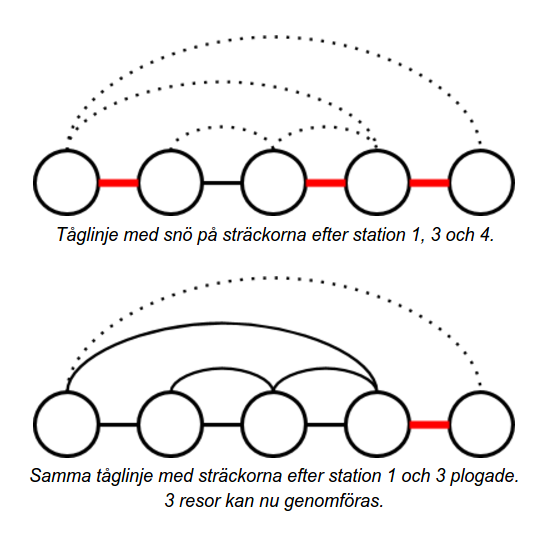
\includegraphics[width=10cm]{snokaos.png}
\caption{Sample 1}
\end{figure} 

\section*{Input}
The first line contains four integers, $2 \le n \le 200$, $ 1 \le m \le 100000 $, $ 0 \le s, p \le n - 1$: the number of stations, the number of travelers, the number of snowed-in sections, and the number of sections Fredrika has time to plow.

Then follow $m$ lines where line $i$ contains two integers $1 \le a_i \not= b_i \le n$, the stations where traveler $i$ wants to start and end.

Then follow $s$ lines where line $j$ contains one integer $ 1 \le c_j \le n - 1$, the station that lies \emph{right before} the snowed-in section $j$.
A section appears at most once in this list.


\section*{Output}
Your program shall output a single integer: the maximum number of travelers that can complete their trips by plowing at most $p$ sections.

\section*{Scoring}
Your solution will be tested on a set of test groups. To earn points for a group, you must pass all test cases in that group.

\begin{tabular}{| l | l | l | l |}
\hline
Group & Points & Constraints & Other \\ \hline
1     & 12         & $ n \le 200, m \le 100, p = 1$ &\\ \hline
2     & 11         & $ n \le 200, m \le 100, s \le 12 $ &\\ \hline
3     & 10          & $ n \le 200, m \le 100$ & $a_i = 1$ for all $a_i$\\ \hline
4     & 67         & $ n \le 200$ &\\ \hline
\end{tabular}
